\documentclass[11pt,a4paper]{article}

% --- Pacotes Essenciais ---
\usepackage[utf8]{inputenc}
\usepackage[T1]{fontenc}
\usepackage[portuguese]{babel}
\usepackage[margin=2.5cm]{geometry}
\usepackage{amsmath,amssymb}
\usepackage{graphicx}
\usepackage{booktabs}
\usepackage{tabularx}
\usepackage{array}
\usepackage{xcolor}
\usepackage{listings}
\usepackage{url}
\usepackage{hyperref}
\usepackage{cite}
\usepackage{setspace}
\onehalfspacing

% Configuracao de Links
\hypersetup{
    colorlinks=true,
    linkcolor=black,
    citecolor=blue,
    urlcolor=blue
}

% Estilo para blocos de codigo e excertos de logs
\lstset{
    basicstyle=\ttfamily\footnotesize,
    breaklines=true,
    frame=single,
    backgroundcolor=\color{gray!8},
    columns=flexible
}

% Macro auxiliar para placeholders de figuras e evidencias
\newcommand{\placeholderfig}[2]{%
    \begin{center}
        \fcolorbox{gray!70}{gray!6}{%
            \parbox{0.92\textwidth}{%
                \vspace{0.5cm}
                \centering
                \textbf{[PLACEHOLDER DE FIGURA: #1]}\\[0.25cm]
                \small \textit{#2}
                \vspace{0.5cm}
            }%
        }
    \end{center}
}

% Macro auxiliar para valores pendentes de preenchimento pos-execucao
\newcommand{\todo}[1]{\textcolor{blue!75!black}{\textbf{[#1]}}}

\begin{document}

% ==========================================
% Capa
% ==========================================
\begin{titlepage}
    \begin{center}
        \vspace*{0.5cm}
        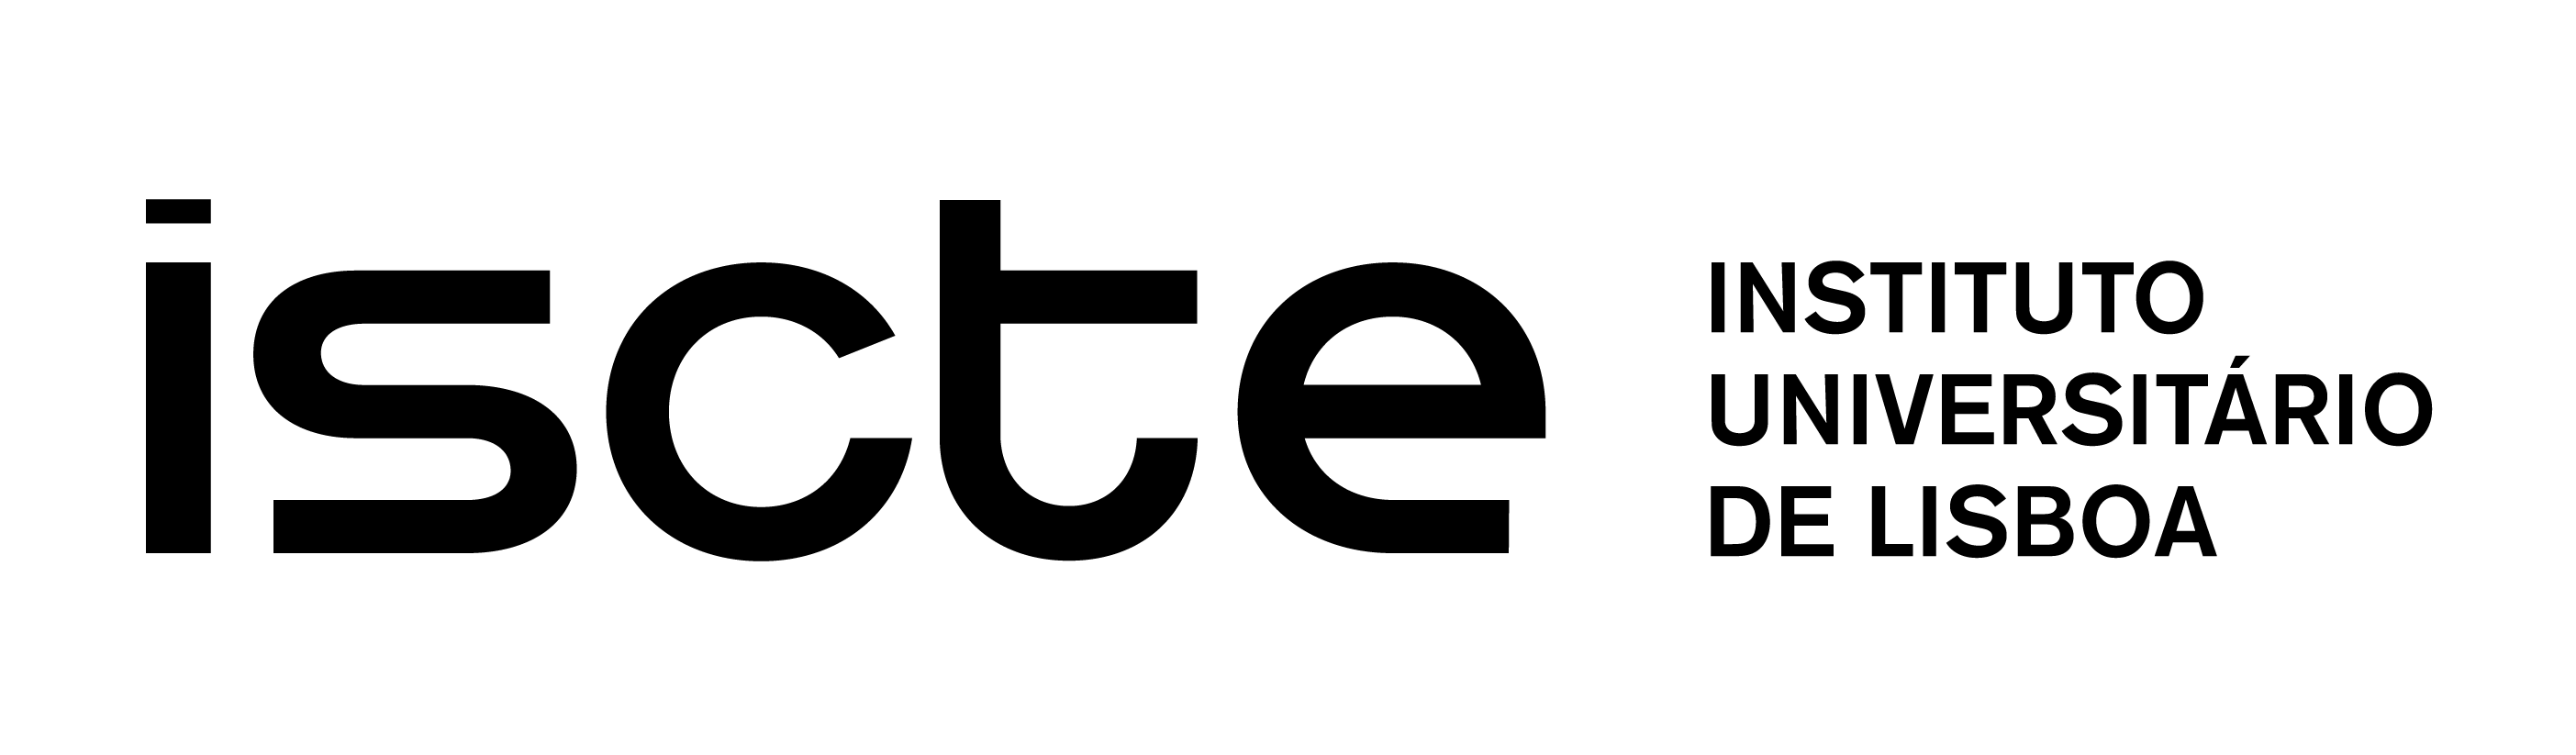
\includegraphics[width=0.65\textwidth]{images/logo-iscte.png}\\[1.5cm]

        {\large Mestrado em Engenharia Informática}\\[0.2cm]
        {\large \textbf{Segurança em Redes e Sistemas de Informação}}\\[1.8cm]

        {\huge \textbf{Análise de Vulnerabilidades Web e Mitigação com \textit{WAF ModSecurity}}}\\[0.5cm]
        {\Large \textbf{Fase 2 --- Implementação Prática e Avaliação Experimental}}\\[1.8cm]

        \large
        \textbf{Autores:}\\[0.3cm]
        Daniel Nunes, Nº 123547\\[0.15cm]
        Guilherme Alves, Nº 122661\\[0.15cm]
        João Oliveira, Nº 142584\\[2cm]

        \textbf{Docente:} Prof. Daniel Caçador\\[0.5cm]
        \textbf{Data:} \today
    \end{center}
\end{titlepage}

% ==========================================
% Resumo
% ==========================================
\clearpage
\section*{Resumo}
\addcontentsline{toc}{section}{Resumo}
Este documento apresenta a segunda fase (componente prática) do projeto de Segurança em Redes e Sistemas de Informação, dando continuidade ao enquadramento teórico e ao modelo formal definidos na Fase 1. Foi implementado um ambiente virtualizado isolado em \textit{Docker} composto pela aplicação intencionalmente vulnerável \textit{Damn Vulnerable Web Application} (DVWA), um \textit{reverse proxy} Nginx sem proteção (\textit{baseline}) e um \textit{reverse proxy} Nginx equipado com o \textit{Web Application Firewall} (WAF) \textit{ModSecurity} v3 e o conjunto de regras OWASP \textit{Core Rule Set} (CRS).

Com recurso a conjuntos reproduzíveis de pedidos maliciosos (\textit{SQL Injection} e \textit{Cross-Site Scripting}, incluindo variantes de evasão) e de tráfego legítimo, bem como às ferramentas \texttt{sqlmap}, \texttt{cURL}, \textit{OWASP ZAP}/\textit{Burp Suite} e \textit{Apache Benchmark} (\texttt{ab}), são avaliadas a eficácia de deteção através da matriz de confusão (Precisão, Sensibilidade, \textit{F1-Score}, Especificidade e Acurácia Balanceada), a análise dos registos estruturados (\texttt{audit.log}) e o impacto na latência ($\Delta L$). \todo{Resumo final a ajustar após recolha dos valores experimentais: ex. taxa global de deteção e $\Delta L$ medido.}

\vspace{0.8cm}
\noindent \textbf{Palavras-chave:} Segurança Web, WAF, \textit{ModSecurity} v3, OWASP CRS, DVWA, \textit{Docker}, \textit{SQL Injection}, XSS, \textit{Benchmarking}.

% ==========================================
% Indice
% ==========================================
\clearpage
\tableofcontents

% ==========================================
% Glossario
% ==========================================
\clearpage
\section*{Glossário}
\addcontentsline{toc}{section}{Glossário}
\begin{description}
    \item[BA] Acurácia Balanceada (\textit{Balanced Accuracy}).
    \item[CRS] \textit{Core Rule Set} (conjunto de regras da OWASP para WAFs).
    \item[DVWA] \textit{Damn Vulnerable Web Application}.
    \item[FN] Falso Negativo (\textit{False Negative}).
    \item[FP] Falso Positivo (\textit{False Positive}).
    \item[OWASP] \textit{Open Web Application Security Project}.
    \item[PL] Nível de Paranoia (\textit{Paranoia Level}) do OWASP CRS.
    \item[RPS] Pedidos por segundo (\textit{Requests Per Second}).
    \item[SQLi] \textit{Structured Query Language Injection}.
    \item[TN] Verdadeiro Negativo (\textit{True Negative}).
    \item[TP] Verdadeiro Positivo (\textit{True Positive}).
    \item[WAF] \textit{Web Application Firewall}.
    \item[XSS] \textit{Cross-Site Scripting}.
\end{description}

% ==========================================
% 1. Introducao
% ==========================================
\clearpage
\section{Introdução}
\label{sec:introducao}

Na primeira fase deste trabalho foram estudados os mecanismos das vulnerabilidades Web críticas \textit{SQL Injection} (SQLi) e \textit{Cross-Site Scripting} (XSS), a arquitetura de inspeção em cinco fases do \textit{ModSecurity} v3 com o OWASP \textit{Core Rule Set} (CRS), e o modelo matemático de avaliação quantitativa baseado na matriz de confusão e no diferencial de latência ($\Delta L$).

A presente segunda fase materializa a prova de conceito desenhada na metodologia da Fase 1. O objetivo central consiste em validar experimentalmente, num ambiente controlado em contentores \textit{Docker}, até que ponto o WAF \textit{ModSecurity} v3 consegue mitigar ataques reais e mutações sintáticas sem comprometer a disponibilidade para utilizadores legítimos nem degradar excessivamente os tempos de resposta.

Em termos específicos, esta fase prática procura responder a quatro questões experimentais:
\begin{enumerate}
    \item As vulnerabilidades alvo (SQLi \textit{In-Band}, SQLi \textit{Blind}, XSS \textit{Reflected} e XSS \textit{Stored}) são efetivamente exploráveis na DVWA na ausência de proteção?
    \item Qual é a eficácia quantitativa do \textit{ModSecurity} v3 + OWASP CRS na configuração padrão (\textit{Paranoia Level 1}) medida através de Precisão, Sensibilidade, \textit{F1-Score}, Especificidade e Acurácia Balanceada?
    \item Como evolui o compromisso entre redução de falsos negativos (evasão) e aumento de falsos positivos ao elevar o nível de paranoia (PL2) e ao aplicar regras personalizadas de afinação (\textit{tuning})?
    \item Qual é a sobrecarga de latência ($\Delta L$) introduzida pela inspeção profunda de pacotes sob diferentes níveis de concorrência?
\end{enumerate}

O restante documento encontra-se organizado da seguinte forma: a Secção \ref{sec:arquitetura} descreve a infraestrutura em \textit{Docker} implementada; a Secção \ref{sec:metodologia_exp} detalha os conjuntos de teste e ferramentas utilizadas; a Secção \ref{sec:resultados} apresenta os resultados experimentais e análise dos registos de auditoria; a Secção \ref{sec:discussao} discute limitações e boas práticas; e a Secção \ref{sec:conclusoes} sintetiza as conclusões finais.

% ==========================================
% 2. Arquitetura e Implementacao do Ambiente
% ==========================================
\clearpage
\section{Arquitetura e Implementação do Ambiente Experimental}
\label{sec:arquitetura}

Para assegurar reprodutibilidade e isolamento durante os ensaios ofensivos, toda a infraestrutura foi definida de forma declarativa em \textit{Docker Compose} na pasta \texttt{SRC/} do repositório do grupo.\footnote{Repositório do projeto: \url{https://github.com/JoaOliveira21/Projeto_SRSI}}

\subsection{Topologia de Contentores e Isolamento de Rede}
O ambiente é composto por três serviços interligados através de uma rede interna dedicada (\texttt{srsi\_net}), com todas as portas publicadas no hospedeiro restringidas exclusivamente à interface local (\texttt{127.0.0.1}) para impedir a exposição da aplicação vulnerável na rede externa:

\begin{itemize}
    \item \textbf{\texttt{dvwa} (\texttt{vulnerables/web-dvwa:latest}):} Contentor com a aplicação alvo \textit{Damn Vulnerable Web Application} (Apache + PHP + MySQL), acessível diretamente em \texttt{127.0.0.1:8081} apenas para verificação inicial do serviço.
    \item \textbf{\texttt{proxy-base} (\texttt{nginx:alpine}):} Servidor Nginx configurado exclusivamente como \textit{reverse proxy} (sem motor WAF) em \texttt{127.0.0.1:8082}, encaminhando o tráfego para \texttt{http://dvwa:80}. A inclusão deste serviço permite medir a linha de base ($L_{\text{Base}}$) em igualdade de arquitetura de \textit{proxy}, isolando estritamente o custo computacional do \textit{ModSecurity} e das regras CRS.
    \item \textbf{\texttt{waf} (\texttt{owasp/modsecurity-crs:nginx}):} Servidor Nginx integrado com o motor \textit{ModSecurity} v3 e o conjunto de regras OWASP CRS, exposto em \texttt{127.0.0.1:8080} e configurado com \texttt{BACKEND=http://dvwa:80}.
\end{itemize}

\begin{figure}[h!]
    \centering
    \placeholderfig{Arquitetura do Ambiente em Docker}{Inserir diagrama da topologia (Cliente / Ferramentas de Teste $\rightarrow$ \texttt{proxy-base:8082} e \texttt{waf:8080} $\rightarrow$ \texttt{dvwa:80} na rede \texttt{srsi\_net}) ou captura de ecrã de \texttt{docker compose ps}.}
    \caption{Arquitetura experimental em contentores \textit{Docker} para avaliação do WAF.}
    \label{fig:arquitetura}
\end{figure}

\subsection{Configuração do \textit{ModSecurity} v3 e Auditoria (Fase 5)}
O comportamento do WAF é parametrizado através do ficheiro \texttt{SRC/.env} e montagens de volume no \texttt{docker-compose.yml}:
\begin{itemize}
    \item \textbf{Modo de Operação:} \texttt{MODSEC\_RULE\_ENGINE=On}, com modo de pontuação de anomalias (\textit{Anomaly Scoring}) configurado com patamares padrão \texttt{ANOMALY\_INBOUND=5} e \texttt{ANOMALY\_OUTBOUND=4}.
    \item \textbf{Nível de Paranoia:} Parametrizado via \texttt{BLOCKING\_PARANOIA} (iniciando em \texttt{1} e posteriormente elevado para \texttt{2} nos ensaios comparativos).
    \item \textbf{Registo de Auditoria:} Configurado com \texttt{MODSEC\_AUDIT\_ENGINE=RelevantOnly}, formato estruturado \texttt{MODSEC\_AUDIT\_LOG\_FORMAT=JSON} e partes \texttt{ABIJDEFHZ}, persistido no volume local \texttt{SRC/logs/audit.log}.
    \item \textbf{Regras Personalizadas:} Montagem dos ficheiros \texttt{REQUEST-900-EXCLUSION-RULES-BEFORE-CRS.conf} e \texttt{RESPONSE-999-EXCLUSION-RULES-AFTER-CRS.conf} para afinação de falsos positivos e adição de assinaturas específicas.
\end{itemize}

% ==========================================
% 3. Metodologia Experimental e Conjuntos de Teste
% ==========================================
\clearpage
\section{Metodologia Experimental e Conjuntos de Teste}
\label{sec:metodologia_exp}

\subsection{Preparação da Aplicação Alvo (DVWA)}
Para garantir condições homogéneas entre os ensaios no \textit{baseline} e no WAF, o script de avaliação automatizado executa previamente os seguintes passos sobre ambos os caminhos HTTP:
\begin{enumerate}
    \item Verificação e inicialização da base de dados da DVWA através do \textit{endpoint} \texttt{/setup.php} (com extração automática do token anti-CSRF \texttt{user\_token}).
    \item Autenticação programática em \texttt{/login.php} com as credenciais padrão (\texttt{admin}/\texttt{password}).
    \item Definição explícita do nível de segurança da DVWA para \texttt{low} via \texttt{/security.php} e respetivo \textit{cookie} de sessão (\texttt{PHPSESSID} e \texttt{security=low}).
\end{enumerate}

\subsection{Desenho dos Conjuntos de Teste (Ataques e Tráfego Legítimo)}
Em conformidade com a formulação matemática da Secção 4 da Fase 1, a validação do WAF exige tanto pedidos maliciosos (para contabilizar $TP$ e $FN$) como pedidos legítimos (para contabilizar $TN$ e $FP$). Foram construídos dois conjuntos determinísticos em formato TSV na pasta \texttt{SRC/datasets/}:

\begin{table}[h!]
\centering
\caption{Composição dos conjuntos de teste utilizados na avaliação automatizada.}
\label{tab:composicao_datasets}
\begin{tabularx}{\textwidth}{l l c X}
\toprule
\textbf{Conjunto / Categoria} & \textbf{\textit{Endpoint} DVWA} & \textbf{Nº Casos} & \textbf{Objetivo / Exemplos de Vetores} \\
\midrule
\texttt{SQLi\_InBand} & \texttt{/vulnerabilities/sqli/} & 6 & Tautologias (\texttt{' OR '1'='1}), extração via \texttt{UNION SELECT} e enumeração (\texttt{ORDER BY}). \\
\texttt{SQLi\_Blind} & \texttt{/vulnerabilities/sqli\_blind/} & 5 & Inferência booleana (\texttt{AND 1=1}) e temporal (\texttt{SLEEP(2)}, \texttt{IF(...,SLEEP(2),0)}). \\
\texttt{SQLi\_Evasion} & \texttt{/vulnerabilities/sqli/} & 4 & Comentários \textit{inline} (\texttt{/**/}), comentários condicionais MySQL (\texttt{/*!50000OR*/}) e tabulação (\texttt{\%09}). \\
\texttt{XSS\_Reflected} & \texttt{/vulnerabilities/xss\_r/} & 4 & \textit{Tags} \texttt{<script>}, eventos \texttt{onerror}/\texttt{onload} e quebra de atributo (\texttt{">}). \\
\texttt{XSS\_Stored} & \texttt{/vulnerabilities/xss\_s/} & 4 & Injeção persistente via \texttt{POST} nos campos \texttt{mtxMessage} e \texttt{txtName}. \\
\texttt{XSS\_Evasion} & \texttt{/vulnerabilities/xss\_r/} & 5 & Mistura de maiúsculas/minúsculas, separador \texttt{/}, \texttt{<details ontoggle>} e codificação em entidades HTML. \\
\midrule
\textbf{Total Ataques} & --- & \textbf{28} & \textbf{Avaliação de $TP$ (HTTP 403) e $FN$ (não bloqueado).} \\
\midrule
\texttt{Legítimo (Normal)} & Todos os anteriores & 16 & IDs numéricos válidos, nomes próprios, \textit{emails} académicos e comentários normais no \textit{Guestbook}. \\
\texttt{Legítimo (Fronteira)} & \texttt{xss\_r}, \texttt{xss\_s} & 4 & Casos realistas suscetíveis de gerar falsos positivos: apóstrofo (\texttt{O'Connor}), operador (\texttt{2 < 5}) e palavras como \textit{select}/\textit{union} em frases naturais. \\
\midrule
\textbf{Total Legítimo} & --- & \textbf{20} & \textbf{Avaliação de $TN$ (permitido) e $FP$ (HTTP 403 indevido).} \\
\bottomrule
\end{tabularx}
\end{table}

\subsection{Ferramentas de Exploração, Inspeção e \textit{Benchmarking}}
Para além do motor de execução em lote (\texttt{scripts/run\_evaluation.py}), o protocolo experimental integra as ferramentas previstas na proposta do projeto:
\begin{itemize}
    \item \textbf{\texttt{sqlmap} (via contentor \texttt{parrotsec/sqlmap}):} Exploração automatizada de SQLi \textit{In-Band} e \textit{Blind} contra \texttt{proxy-base} e \texttt{waf} com \textit{cookie} autenticado.
    \item \textbf{\texttt{cURL} e \textit{OWASP ZAP} / \textit{Burp Suite}:} Validação manual de respostas HTTP, interceção de pedidos e verificação interativa de alertas.
    \item \textbf{\textit{Apache Benchmark} (\texttt{ab} via \texttt{httpd:alpine} / \texttt{scripts/run\_benchmark.py}):} Medição comparativa de latência média e pedidos por segundo ($N=500$ pedidos, concorrências $c=10$ e $c=50$) no \textit{endpoint} \texttt{/vulnerabilities/sqli/?id=1\&Submit=Submit}.
\end{itemize}

% ==========================================
% 4. Resultados Experimentais e Analise
% ==========================================
\clearpage
\section{Resultados Experimentais e Análise}
\label{sec:resultados}

\subsection{Validação da Linha de Base (Sem WAF)}
Numa primeira etapa, todos os 28 vetores de ataque foram submetidos através do \textit{proxy} sem proteção (\texttt{http://127.0.0.1:8082}). Confirmou-se que os pedidos maliciosos atingiram a DVWA com código de resposta HTTP \todo{200}, permitindo:
\begin{itemize}
    \item A enumeração de utilizadores e \textit{hashes} da base de dados através de SQLi \textit{In-Band} (\texttt{ATK-03}, \texttt{ATK-04}) e com recurso ao \texttt{sqlmap};
    \item A indução de atrasos de \todo{$\approx 2$ segundos} nos ataques \textit{Time-Based Blind} (\texttt{ATK-09}, \texttt{ATK-10});
    \item A reflexão e persistência de código JavaScript arbitrário nos módulos de XSS \textit{Reflected} e \textit{Stored}.
\end{itemize}

\begin{figure}[h!]
    \centering
    \placeholderfig{Evidência de Exploração Baseline (Sem WAF)}{Inserir captura de ecrã do \texttt{sqlmap} a enumerar bases de dados/tabelas da DVWA sem WAF ou resposta \texttt{cURL} / navegador a comprovar execução de SQLi e XSS em \texttt{proxy-base:8082}.}
    \caption{Exploração bem-sucedida da DVWA na ausência do WAF (\textit{Baseline}).}
    \label{fig:baseline_exploit}
\end{figure}

\subsection{Eficácia de Deteção e Matriz de Confusão (\textit{Paranoia Level 1})}
Com o WAF ativo (\texttt{MODSEC\_RULE\_ENGINE=On}, \texttt{BLOCKING\_PARANOIA=1}), executou-se o conjunto completo de 48 pedidos (28 ataques e 20 legítimos). Os resultados obtidos a partir de \texttt{results/metrics\_summary.json} e \texttt{results/detailed\_results.csv} encontram-se sintetizados nas Tabelas \ref{tab:matriz_confusao_pl1}, \ref{tab:metricas_pl1} e \ref{tab:resultados_categoria}.

\begin{table}[h!]
\centering
\caption{Matriz de confusão obtida com OWASP CRS em \textit{Paranoia Level 1}.}
\label{tab:matriz_confusao_pl1}
\begin{tabular}{l c c c}
\toprule
 & \textbf{Bloqueado pelo WAF (HTTP 403)} & \textbf{Permitido pelo WAF} & \textbf{Total} \\
\midrule
\textbf{Ataque Real (28)} & $TP = \todo{XX}$ & $FN = \todo{XX}$ & 28 \\
\textbf{Tráfego Legítimo (20)} & $FP = \todo{XX}$ & $TN = \todo{XX}$ & 20 \\
\bottomrule
\end{tabular}
\end{table}

\begin{table}[h!]
\centering
\caption{Métricas formais de eficácia do WAF (\textit{Paranoia Level 1}).}
\label{tab:metricas_pl1}
\begin{tabularx}{\textwidth}{l c X}
\toprule
\textbf{Métrica} & \textbf{Valor Obtido} & \textbf{Interpretação Experimental} \\
\midrule
Precisão ($\frac{TP}{TP + FP}$) & \todo{0.XXXX} & Fração dos bloqueios que corresponderam a ataques reais. \\
Sensibilidade / \textit{Recall} ($\frac{TP}{TP + FN}$) & \todo{0.XXXX} & Percentagem do total de ataques efetivamente travada. \\
\textit{F1-Score} & \todo{0.XXXX} & Média harmónica entre Precisão e Sensibilidade. \\
Especificidade ($\frac{TN}{TN + FP}$) & \todo{0.XXXX} & Capacidade de permitir tráfego legítimo sem bloqueios indevidos. \\
Acurácia Balanceada (BA) & \todo{0.XXXX} & Desempenho equilibrado entre deteção de ataques e usabilidade. \\
\bottomrule
\end{tabularx}
\end{table}

\begin{table}[h!]
\centering
\caption{Desagregação dos resultados por categoria de teste (\textit{Paranoia Level 1}).}
\label{tab:resultados_categoria}
\begin{tabular}{l c c c c c}
\toprule
\textbf{Categoria} & \textbf{Total} & \textbf{TP / TN} & \textbf{FN / FP} & \textbf{Taxa de Sucesso (\%)} & \textbf{Observações} \\
\midrule
\texttt{SQLi\_InBand} & 6 & \todo{X} & \todo{X} & \todo{XX.X\%} & \todo{Ex: bloqueado por regras 942xxx} \\
\texttt{SQLi\_Blind} & 5 & \todo{X} & \todo{X} & \todo{XX.X\%} & \todo{Ex: SLEEP/booleano bloqueado} \\
\texttt{SQLi\_Evasion} & 4 & \todo{X} & \todo{X} & \todo{XX.X\%} & \todo{Indicar se houve bypass} \\
\texttt{XSS\_Reflected} & 4 & \todo{X} & \todo{X} & \todo{XX.X\%} & \todo{Ex: bloqueado por regras 941xxx} \\
\texttt{XSS\_Stored} & 4 & \todo{X} & \todo{X} & \todo{XX.X\%} & \todo{Inspeção do corpo POST (Fase 2)} \\
\texttt{XSS\_Evasion} & 5 & \todo{X} & \todo{X} & \todo{XX.X\%} & \todo{Indicar eventuais FN} \\
\texttt{Legítimo (Normal + Fronteira)} & 20 & \todo{X} & \todo{X} & \todo{XX.X\%} & \todo{Indicar eventuais FP em LEG-17..20} \\
\bottomrule
\end{tabular}
\end{table}

\begin{figure}[h!]
    \centering
    \placeholderfig{Bloqueio de Ferramentas Automatizadas pelo WAF}{Inserir captura de ecrã do \texttt{sqlmap} a ser bloqueado (HTTP 403 / deteção de WAF) e/ou do \textit{OWASP ZAP}/\textit{Burp Suite} face a \texttt{waf:8080}.}
    \caption{Comportamento de ferramentas automatizadas de ataque perante o WAF ativo.}
    \label{fig:waf_tools}
\end{figure}

\subsection{Análise de Evasão, \textit{Paranoia Levels} e Afinação (\textit{Tuning})}
Para avaliar empiricamente o compromisso entre segurança e falsos positivos descrito na literatura, repetiu-se a avaliação elevando \texttt{BLOCKING\_PARANOIA=2} e, posteriormente, aplicando regras de exceção/afinação em \texttt{SRC/modsecurity/}. A Tabela \ref{tab:comparacao_pl} compara os três cenários.

\begin{table}[h!]
\centering
\caption{Comparação de desempenho do WAF entre \textit{Paranoia Level 1}, \textit{Level 2} e pós-\textit{tuning}.}
\label{tab:comparacao_pl}
\begin{tabular}{l c c c c c c}
\toprule
\textbf{Configuração} & \textbf{TP} & \textbf{FN} & \textbf{FP} & \textbf{TN} & \textbf{Sensibilidade} & \textbf{Especificidade} \\
\midrule
OWASP CRS PL1 (Padrão) & \todo{X} & \todo{X} & \todo{X} & \todo{X} & \todo{0.XXXX} & \todo{0.XXXX} \\
OWASP CRS PL2 & \todo{X} & \todo{X} & \todo{X} & \todo{X} & \todo{0.XXXX} & \todo{0.XXXX} \\
OWASP CRS PL2 + \textit{Tuning} & \todo{X} & \todo{X} & \todo{X} & \todo{X} & \todo{0.XXXX} & \todo{0.XXXX} \\
\bottomrule
\end{tabular}
\end{table}

\todo{Descrever aqui quais os casos concretos de \texttt{attacks.tsv} que geraram FN em PL1 (se houver) e quais os casos de \texttt{legitimate.tsv} (ex.: \texttt{LEG-17}, \texttt{LEG-18} ou \texttt{LEG-19}) que geraram FP em PL2, explicando a regra de exceção (\texttt{ctl:ruleRemoveTargetById} ou \texttt{ctl:ruleRemoveById}) adicionada em \texttt{RESPONSE-999-EXCLUSION-RULES-AFTER-CRS.conf}.}

\subsection{Análise dos Registos de Auditoria (\texttt{audit.log})}
Na Fase 5 do ciclo de vida do \textit{ModSecurity}, todas as transações relevantes foram registadas em formato JSON em \texttt{SRC/logs/audit.log}. A Tabela \ref{tab:top_regras_crs} lista as regras do OWASP CRS mais frequentemente ativadas durante os ensaios.

\begin{table}[h!]
\centering
\caption{Regras do OWASP CRS com maior número de ativações no \texttt{audit.log}.}
\label{tab:top_regras_crs}
\begin{tabularx}{\textwidth}{c c X c}
\toprule
\textbf{ID da Regra} & \textbf{Fase} & \textbf{Descrição / Mensagem} & \textbf{Ocorrências} \\
\midrule
\todo{942100} & \todo{2} & \todo{SQL Injection Attack Detected via libinjection} & \todo{XX} \\
\todo{941100} & \todo{2} & \todo{XSS Attack Detected via libinjection} & \todo{XX} \\
\todo{949110} & \todo{2} & \todo{Inbound Anomaly Score Exceeded (Total Score: ...)} & \todo{XX} \\
\todo{...} & \todo{...} & \todo{Adicionar restantes regras de \texttt{metrics\_summary.json}} & \todo{XX} \\
\bottomrule
\end{tabularx}
\end{table}

O excerto seguinte ilustra um evento real extraído de \texttt{audit.log}, evidenciando o mecanismo de \textit{Anomaly Scoring} até ao bloqueio final com HTTP \texttt{403}:

\begin{lstlisting}[caption={Excerto do registo JSON em \texttt{SRC/logs/audit.log} (substituir por excerto real).},label={lst:audit_json}]
{
  "transaction": {
    "client_ip": "172.18.0.1",
    "request": {
      "method": "GET",
      "uri": "/vulnerabilities/sqli/?id=1'+OR+'1'%3D'1&Submit=Submit"
    },
    "response": { "http_code": 403 },
    "messages": [
      {
        "message": "[PLACEHOLDER: substituir pelo JSON real obtido em SRC/logs/audit.log]",
        "details": { "ruleId": "942100", "severity": "2" }
      }
    ]
  }
}
\end{lstlisting}

\subsection{Avaliação de Desempenho e Impacto na Latência ($\Delta L$)}
Para quantificar a sobrecarga introduzida pelo motor de inspeção de acordo com a Equação $\Delta L = L_{\text{WAF}} - L_{\text{Base}}$, executou-se o \textit{Apache Benchmark} (\texttt{ab}) sobre $N = 500$ pedidos autenticados ao \textit{endpoint} \texttt{/vulnerabilities/sqli/?id=1\&Submit=Submit} para dois níveis de concorrência ($c=10$ e $c=50$). Os valores recolhidos em \texttt{results/latency\_benchmark.csv} são apresentados na Tabela \ref{tab:benchmark_latencia}.

\begin{table}[h!]
\centering
\caption{Comparação de latência e débito entre Nginx sem WAF ($L_{\text{Base}}$) e com ModSecurity ($L_{\text{WAF}}$).}
\label{tab:benchmark_latencia}
\begin{tabular}{c c c c c c c}
\toprule
\textbf{Concorrência ($c$)} & \textbf{$L_{\text{Base}}$ (ms)} & \textbf{$L_{\text{WAF}}$ (ms)} & \textbf{$\Delta L$ (ms)} & \textbf{Sobrecarga (\%)} & \textbf{Base (RPS)} & \textbf{WAF (RPS)} \\
\midrule
10 & \todo{XX.XX} & \todo{XX.XX} & \todo{+XX.XX} & \todo{+XX.X\%} & \todo{XXX.X} & \todo{XXX.X} \\
50 & \todo{XX.XX} & \todo{XX.XX} & \todo{+XX.XX} & \todo{+XX.X\%} & \todo{XXX.X} & \todo{XXX.X} \\
\bottomrule
\end{tabular}
\end{table}

\begin{figure}[h!]
    \centering
    \placeholderfig{Comparação de Latência e RPS ($L_{\text{Base}}$ vs. $L_{\text{WAF}}$)}{Inserir gráfico de barras comparando o tempo médio de resposta (ms) e o percentil $p_{95}$ ou RPS para $c=10$ e $c=50$.}
    \caption{Impacto do WAF \textit{ModSecurity} v3 na latência média e capacidade de processamento.}
    \label{fig:latencia_comparacao}
\end{figure}

% ==========================================
% 5. Discussao Critica e Limitacoes
% ==========================================
\clearpage
\section{Discussão Crítica e Limitações}
\label{sec:discussao}

Com base nas observações efetuadas durante os testes práticos, destacam-se os seguintes aspetos críticos:
\begin{enumerate}
    \item \textbf{Defesa em Profundidade vs. Correção na Origem:} Embora o \textit{ModSecurity} v3 + OWASP CRS bloqueie eficazmente a maioria das explorações de SQLi e XSS antes de atingirem a aplicação PHP, a vulnerabilidade subjacente na DVWA permanece presente. Um WAF atua como camada compensatória e de mitigação imediata, não substituindo o uso de \textit{prepared statements} nem a codificação contextual de saída.
    \item \textbf{Limitações de Assinaturas e Evasão:} \todo{Comentar o comportamento observado nos casos \texttt{SQLi\_Evasion} e \texttt{XSS\_Evasion}, explicando porque determinadas mutações sintáticas ou codificações exigem normalizações adicionais ou níveis de paranoia superiores.}
    \item \textbf{Compromisso Operacional e \textit{Tuning}:} O aumento do nível de paranoia reduz o risco de falsos negativos, mas aumenta a sensibilidade a entradas legítimas com caracteres especiais (como apóstrofos ou operadores matemáticos). A análise sistemática do \texttt{audit.log} revela-se indispensável para criar exclusões cirúrgicas por \textit{URI} e parâmetro sem desativar a proteção global.
    \item \textbf{Custo de Desempenho:} \todo{Discutir se o $\Delta L$ medido na Tabela \ref{tab:benchmark_latencia} é aceitável para aplicações Web típicas e como escala entre $c=10$ e $c=50$ pedidos concorrentes.}
    \item \textbf{Validade e Âmbito dos Testes:} Os ensaios decorreram em ambiente local virtualizado com um conjunto controlado de 48 pedidos (28 ataques e 20 pedidos legítimos) sobre quatro módulos da DVWA em nível \textit{low}, sem cifragem TLS nem tráfego de produção complexo (ex.: \textit{payloads} JSON extensos).
\end{enumerate}

% ==========================================
% 6. Conclusoes e Trabalho Futuro
% ==========================================
\clearpage
\section{Conclusões e Trabalho Futuro}
\label{sec:conclusoes}

A segunda fase do projeto permitiu validar experimentalmente o papel do \textit{Web Application Firewall} \textit{ModSecurity} v3 integrado em Nginx com o OWASP \textit{Core Rule Set} na proteção de uma aplicação Web vulnerável (DVWA) em ambiente \textit{Docker}.

Os ensaios demonstraram que, na ausência do WAF, os vetores de \textit{SQL Injection} e \textit{Cross-Site Scripting} são explorados com sucesso, ao passo que a ativação do WAF alcançou uma Sensibilidade de \todo{XX.X\%}, uma Especificidade de \todo{XX.X\%} e um \textit{F1-Score} de \todo{0.XXXX} em \textit{Paranoia Level 1}, introduzindo uma sobrecarga média de latência $\Delta L$ de \todo{+XX.XX ms} para concorrência $c=10$ e \todo{+XX.XX ms} para $c=50$. A análise dos registos em \texttt{audit.log} confirmou o funcionamento do modelo de \textit{Anomaly Scoring} e permitiu fundamentar decisões de afinação de regras.

Como trabalho futuro, identificam-se três linhas de evolução natural:
\begin{itemize}
    \item Integração de inspeção sobre tráfego cifrado HTTPS/TLS e APIs REST/JSON com validação de esquemas (\textit{OpenAPI});
    \item Comparação direta com abordagens de modelo positivo (\textit{NAXSI}) ou classificação assistida por \textit{Machine Learning} para deteção de mutações \textit{zero-day};
    \item Automatização contínua dos testes de regressão de segurança em \textit{pipelines} CI/CD antes da publicação de novas regras de WAF em produção.
\end{itemize}

% ==========================================
% Referencias
% ==========================================
\clearpage
\begin{thebibliography}{99}

\bibitem{owasp_top10}
OWASP Foundation, ``OWASP Top 10: The Ten Most Critical Web Application Security Risks,'' \url{https://owasp.org/www-project-top-ten/}, 2021.

\bibitem{modsec_crs}
C. Folini and W. Blume, \textit{OWASP ModSecurity Core Rule Set (CRS) Official Documentation}, OWASP Foundation, 2023.

\bibitem{modsec_v3}
Trustwave SpiderLabs / OWASP, ``ModSecurity v3 (libmodsecurity) Reference Manual,'' \url{https://github.com/owasp-modsecurity/ModSecurity}, 2024.

\bibitem{dvwa}
R. Dewhurst et al., ``Damn Vulnerable Web Application (DVWA),'' \url{https://github.com/digininja/DVWA}, 2024.

\bibitem{sqlmap}
B. Damele and M. Stampar, ``sqlmap: Automatic SQL Injection and Database Takeover Tool,'' \url{https://sqlmap.org/}, 2024.

\bibitem{ab_apache}
Apache Software Foundation, ``ab --- Apache HTTP Server Benchmarking Tool,'' \url{https://httpd.apache.org/docs/current/programs/ab.html}, 2024.

\bibitem{alenezi2020}
M. Alenezi and H. S. S. Al-Dhafer, ``Effectiveness of Web Application Firewalls: A Comparative Study of Open-Source Solutions,'' \textit{International Journal of Advanced Computer Science and Applications (IJACSA)}, vol. 11, no. 5, pp. 245--252, 2020.

\bibitem{varghese2019}
A. Varghese and T. Jacob, ``Performance and Latency Evaluation of Web Application Firewalls in Cloud and Virtualized Environments,'' \textit{Journal of Information Security and Applications}, vol. 48, pp. 102--111, 2019.

\end{thebibliography}

\end{document}
